\section{Software}
\label{sec:software}

Collecting a sufficiently large dataset of pictures is not trivial.
% Why is it not trivial?
When done manually, the camera has to be started and stopped for each throw.
This likely creates many empty frames at the beginning and at the end of the capture.
Those empty and therefore invalid frames must be removed to avoid errors during the training of the CNN later on.
Furthermore, each valid frame must be labeled.
This procedure is very error-prone if it is performed manually for each individual frame.
% Solution
To simplify this task, a camera throw detection mechanism is implemented and various Python scripts are used.

This chapter desrcibes the camera interface, the implemented throw detection mechanism, the used database and the various Python scripts.

\subsection{Camera Inteface}
\label{subsec:camera_interface}
% \todo[inline]{}

Baumer provides the Baumer Generic Application Programming Interface (Baumer GAPI) to control its industrial cameras.
The Baumer GAPI supports the programming languages C\# and C++. For performance reasons C++ was used.

This section provides an overview of the Baumer GAPI, the available pixel formats and the camera connection interface USB3 Vision.

\subsubsection{Baumer GAPI Overview}
\label{subsubsec:baumer_gapi_overview}
% \todo[inline]{Citations}
% Baumer GAPI Programmers Guide (needs to be downloaded)

% The Baumer GAPI provides main classes that represent the logical and physical components of the image processing system.
% The Baumer GAPI is based on the Generic Interface for Cameras (GenICam) and provides main classes that represent the logical and physical components of the image processing system.
% The Baumer GAPI is a package of several libraries and is based on the Generic Interface for Cameras (GenICam).
The Baumer GAPI is based on the Generic Interface for Cameras (GenICam).
It is a package of several libraries and the GenICam Producers (e.g. \texttt{bgapi2\_usb.cti}).
% It is a package of several libraries and the so-called Producer files (e.g. \texttt{bgapi2\_usb.cti}).
% The Producer file (e.g. \texttt{bgapi2\_usb.cti}) provides the main classes that represent the logical and physical components of the image processing system.
It provides the main classes that represent the logical and physical components of the image processing system.
Furthermore, it provides list classes to enable discovery and listing of the main objects.
There are even some additional classes to transform images and for debugging.
All classes are available through the namespace \texttt{BGAPI2} after including the header file \texttt{bgapi2\_genicam.hpp}.
% https://www.baumer.com/ch/en/product-overview/industrial-cameras-image-processing/software/baumer-gapi-sdk/c/14174

\begin{table}[hb]
  \caption{Overview of the most important Baumer GAPI classes}
  \label{tab:baumer_gapi}
  \centering
  \begin{tabular}{llp{8.5cm}}
    \toprule
    \textbf{Main Classes} & \textbf{List Classes} & \textbf{Description} \\
    \midrule
     & \textbf{\texttt{SystemList}} & The \texttt{SystemList} class is used to discover objects of the \texttt{System} class (Producer) \\
    \midrule
    \textbf{\texttt{System}} & \textbf{\texttt{InterfaceList}} & The \texttt{System} class is the abstraction of the Producer and used to discover objects of the \texttt{Interface} class \\
    \midrule
    \textbf{\texttt{Interface}} & \textbf{\texttt{DeviceList}} & The Interface class represents a physical interface (e.g. USB) and can be used to discover objects of the \texttt{Device} class \\
    \midrule
    \textbf{\texttt{Device}} & \textbf{\texttt{DataStream}} & The device class is used to configure the camera and can be used to discover objects of the \texttt{DataStream} class \\
    \midrule
    \textbf{\texttt{DataStream}} & \textbf{\texttt{BufferList}} & This class represents a data stream from the camera to the host and can be used to discover objects of the \texttt{Buffer} class \\
    \midrule
    \textbf{\texttt{Buffer}} &  & The \texttt{Buffer} class encapsulates a single memory buffer \\
    \bottomrule
  \end{tabular}
\end{table}

\subsubsection{Pixel Formats}
\label{subsubsec:pixel_format}
% \todo[inline]{Citations, Document, that only 8bits are used? No.}
% (https://en.ids-imaging.com/tl_files/downloads/techtip/TechTip_18MP-color-sensor-as-mono_EN.pdf)

The Baumer industrial camera VCXU-13C uses the digital image sensor PYTHON1300 from ON Semiconductor and allows for the use of monochrome, raw and color pixel formats (see chapter \ref{sec:camera}).
The digital image sensor itself has 1280 $\times$ \SI{1024}{px} that acquire brightness with a bit depth of \SI{10}{bit}.
In order to capture color images, a color filter is applied to each individual pixel.
These red, green and blue (RGB or BGR) color filters only transmit light with a particular wavelength.
Due to the fact that the luminance perception of the human eye is most sensitive to green light, twice as many green filters are used as red and blue filters.
The color filters are arranged in a Bayer color matrix $B$, as shown in figure \ref{subfig:bayerrg} \cite{dcs}.

There are several modifications of the Bayer pattern that can be achieved by simply shifting the pixels around.
The pattern in figure \ref{subfig:bayergr} is achieved by shifting the initial pattern one pixel to the left, whereas the pattern in figure \ref{subfig:bayergb} is achieved by shifting the pattern one pixel up.

The different Bayer patterns are usually named after the color of the elements $B_{1,1}$, $B_{1,2}$, $B_{2,1}$ and $B_{2,2}$.
This results in the four possible patterns \texttt{RGGB}, \texttt{GRBG}, \texttt{GBRG} and \texttt{BGGR}.

However, there exist different naming conventions for the different Bayer patterns.
Baumer labels the Bayer patterns after the color of the elements $B_{1,1}$ and $B_{1,2}$, resulting in the name \texttt{BayerRG} for figure \ref{subfig:bayerrg}.
The Open Computer Vision Library (OpenCV) labels them after the elements $B_{2,2}$ and $B_{2,3}$, resulting in the name \texttt{BayerBG} for the same figure \ref{subfig:bayerrg} \cite{baumer_opencv}.

In order to create an RGB color image from the raw Bayer pattern image, a demosaicing (also ``debayering'') algorithm is necessary.
The Baumer industrial camera VCXU-13C is able to transform the raw sensor data into the respective RGB or BGR values in real time.
Another possibility is to do the required color space transformation with the OpenCV function \texttt{cv::cvtColor}.
Since OpenCV uses the BGR instead of the standard RGB color space, the required color space conversion code is \texttt{cv::COLOR\_BayerBG2BGR}.
This will convert the raw Bayer pattern image into a BGR image \cite{opencv_csc}.

\begin{figure}[ht]
  \centering
  \begin{subfigure}[b]{0.3\textwidth}
    \centering
    \includegraphics[scale=1]{bayerrg}
    \caption{\texttt{RGGB} (Baumer \texttt{BayerRG})}
    \label{subfig:bayerrg}
  \end{subfigure}
  \begin{subfigure}[b]{0.3\textwidth}
    \centering
    \includegraphics[scale=1]{bayergr}
    \caption{\texttt{GRBG} (Baumer \texttt{BayerGR})}
    \label{subfig:bayergr}
  \end{subfigure}
  \begin{subfigure}[b]{0.3\textwidth}
    \centering
    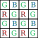
\includegraphics[scale=1]{bayergb}
    \caption{\texttt{GBRG} (Baumer \texttt{BayerGB})}
    \label{subfig:bayergb}
  \end{subfigure}
  \caption{Bayer color matrices $B$}
  \label{fig:bayer}
\end{figure}

\clearpage
\subsubsection{USB3 Vision Interface}
\label{subsubsec:usb3_vision_interface}
% \todo[inline]{Citations (GAPI for leader), Table position}

The Baumer industrial camera VCXU-13C uses the USB3 Vision (U3V) interface with a maximum transfer rate of \SI{5}{Gbit/s} $\approx$ \SI{596}{MiB}.
The max. frame rate is \SI{222}{fps} and the total pixel count is equal to
\[
\text{Pixel}_\text{tot} = \text{Pixel}_\text{width} \cdot \text{Pixel}_\text{height} = \SI{1280}{px} \cdot \SI{1024}{px} = \SI{1310720}{px}.
\]

To calculate the required data rate in bytes per second, equation \ref{eq:data_rate} can be used.
Baumer transmits further information in addition to the actual image data (e.g. frame id, width and height).
This metadata is located in the so-called leader and can be neglected in the calculations due to its relatively small size.
% https://www.baumer.com/ch/en/product-overview/industrial-cameras-image-processing/software/baumer-gapi-sdk/c/14174

\begin{equation}
  \text{Req. data rate} = \text{Pixel}_\text{tot} \cdot \text{Bytes per pixel} \cdot \text{Frame rate}
  \label{eq:data_rate}
\end{equation}

For this application a fixed frame rate of \SI{200}{fps} is sufficient and facilitates the calculations.

Table \ref{tab:data_rates} shows the required data rates for the Baumer pixel format \texttt{BayerRG8} and \texttt{BGR8}.
It is evident that due to the maximum transfer rate of \SI{596}{MiB} of the U3V interface, only the Baumer \texttt{BayerRG8} pixel format is suitable.
% https://www.baumer.com/ch/de/produktubersicht/industriekameras-bildverarbeitung/industriekameras/cx-serie/usb-3-0-schnittstelle/vcxu-13c/p/23792

\begin{table}[h]
  \caption{Required data rate for the two Baumer pixel formats \texttt{BayerRG8} and \texttt{BGR8}}
  \label{tab:data_rates}
  \centering
  \begin{tabular}{lll}
    \toprule
     & \textbf{\texttt{BayerRG8}} & \textbf{\texttt{BGR8}} \\
    \midrule
    \textbf{Bytes per pixel} & \SI{1}{B} & \SI{3}{B} \\
    \textbf{Frame rate} & \SI{200}{fps} & \SI{200}{fps} \\
    \textbf{Req. data rate} & \SI{250}{MiB/s} & \SI{750}{MiB/s} \\
    \bottomrule
  \end{tabular}
\end{table}

\subsubsection{Camera Configuration}
\label{subsubsec:camera_configuration}
% \todo[inline]{}

The camera configuration should be the same during data collection and deployment.
For this reason, the optimal parameters have been carefully selected.
Table \ref{tab:config} lists the important configurations and their respective values.

\begin{table}[hb]
  \caption{Camera configuration}
  \label{tab:config}
  \centering
  \begin{tabular}{lll}
    \toprule
    \textbf{Parameter} & \textbf{Value} & \textbf{Description} \\
    \midrule
    BalanceWhiteAuto & \texttt{Once} & Perform the white balance once during setup \\
    Gain & 4 & For the max. brightness, the max. gain is used \\
    ExposureTime & \SI{250}{\micro\second} & A short exposure time of \SI{250}{\micro\second} is used \\
    AcquisitionFrameRateEnable & \texttt{true} & Enable fixed frame rate \\
    AcquisitionFrameRate & \SI{200}{fps} & Set fixed frame rate to \SI{200}{fps} \\
    TriggerMode & \texttt{Off} & Use no trigger (free run) \\
    PixelFormat & \texttt{BayerRG8} & Use the raw Baumer \texttt{BayerRG8} pixel format \\
    \bottomrule
  \end{tabular}
\end{table}

\clearpage

\subsection{Throw Detection Mechanism}
\label{subsec:throw_detection_mechanism}

To reliably detect a throw, a simple image change detection algorithm is implemented.
It requires a repeated difference computation and therefore a circular buffer is used.

This section explains the employed algorithm, its implementation and the saving of the images.

% \subsubsection{Image Change Detection Algorithm}
% \subsubsection{Throw Detection Algorithm}
\subsubsection{Employed Algorithm}
\label{subsubsec:algorithm}
% \todo[inline]{No citations?! Or OpenCV?! Or Baumer?!}

% image change detection algorithm vs throw detection / throw detection mechanism / throw detection algorithm => throw detection employs icda

% Goal of the throw detection is to extract the valid frames of a throw from the continous data stream
  % valid frames have object on them, invalid frames are empty (background)
% real-time
% serial process, 200 fps => >5 ms to process each frame
% not a lot of time for a complex (fancy) algorithm => simplest one possible is used
  % for the throw detection algorithm a simple image change detection algorithm is used

% Algo: computation of the difference and comparison to a threshold to detect changes in the picture

% what this sections does with the listings

% Due to the in section {} mentioned bandwidth limitations of the U3V interface the raw bayer is processed
  % conversion to BGR8 takes too long! => use raw bayer for the detection
% Saving images takes time + unnecessary => saving at the end!
  % see section \ref

% buffers

% frame_id (FID) to keep track of ...
% uses 2 flags and 2 "pointers" to the buffer

% compared against threshold (if mean_diff < threshold, considered to be no change [equal sign])

% throw begin and throw end, what happens

% Why are the last two frames are not valid?
  % only possible to detect the end when there is no change any longer

The goal of the throw detection is to extract valid frames of a throw --- with objects on them --- from the continous data stream of the camera.
Therefore, the throw detection needs to work in real time.
At a frame rate of \SI{200}{fps}, there is $<\SI{5}{ms}$ to process a single frame (without the use of parallel computing).
Due to this time constraint, a simple image change detection algorithm is employed.

\paragraph{Image Change Detection Algorithm}
\vspace{-20pt}
\begin{enumerate}
  \item Compute the absolute difference between the current and the last frame
  \item Compute the average among all the pixels of the difference
  \item Compare the mean difference against a threshold value
\end{enumerate}

This section describes only selected parts of the implementation.
The complete listing of the throw detection can be found in appendix \ref{app:throw_detection}.
The implementation of the difference computation and the average among all the pixels is described in section \ref{subsubsec:difference_computation}.
Furthermore, the way the threshold value is obtained is documented in section \ref{subsubsec:threshold}.

Due to the bandwidth limitations of the U3V interface mentioned in section \ref{subsubsec:usb3_vision_interface}, the received images are in the raw Bayer pixel format.
A conversion from the Baumer \texttt{BayerRG8} to \texttt{BGR8} takes too long an therefore the raw frames are processed.
Moreover, the valid images are only saved on the hard disk at the end of a throw, as this also takes a lot of time (see section \ref{subsubsec:saving_images}).

For the above reasons, two image buffers are used.
The received images are stored in Baumer \texttt{BGAPI2::Buffer} objects (see section \ref{subsubsec:baumer_buffer}).
To save the images later on, a circular buffer for OpenCV matrices (\texttt{cv::Mat}) is used.
This is documented in section \ref{subsubsec:opencv_buffer}.
The size of those image buffers (\texttt{BS}) determines the max. amount of valid frames $N_\text{max}$ that can be captured.

To keep track of the present and past frames, a frame id (\texttt{FID}) is utilized.
Furthermore, two flags are used to mark the beginning and the end of a throw.

Whenever the mean difference between two consecutive frames is greater than or equal to the threshold, they are considered to be different ($\ne$).
Otherwise, the two frames are considered to be equal ($=$).

Once two consecutive frames are different, the flag \texttt{throw\_bgn} is set to \texttt{true} and the current \texttt{FID} is saved in \texttt{throw\_bgn\_idx}.
The current and all subsequent frames --- except for the last two --- belong to the detected throw until two consecutive frames are no longer different.
In this case, the flag \texttt{throw\_end} is set to \texttt{true} and the current \texttt{FID} is saved in \texttt{throw\_end\_idx}.

The last two frames are not valid due to the way the throw detection works.
The first invalid frame occurs when the object leaves the image, as this is still a change in the image and thus not detected.
The second invalid frame results from the fact that the following images are only now the same and therefore the current \texttt{FID} is saved.

Figure \ref{subfig:algorithm_general_case} shows the general case of the just described throw detection.
As already mentioned, the max. amount of valid frames $N_\text{max}$ depends on the image buffer size (\texttt{BS}).
To properly detected a throw, the amount of valid frames $N$ must meet the condition
\[
  N \in \{1..(\text{BS}-2)\}.
\]
In the current implementation, an image buffer size of \SI{1000}{} is used and therefore $N_\text{max} = \SI{998}{frames}$.
An example of three valid frames ($N = 3$) is shown in figure \ref{subfig:algorithm_example_3}.

\begin{figure}[H]
  \centering
  \begin{subfigure}[b]{\textwidth}
    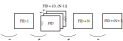
\includegraphics[scale=0.85]{algorithm}
    \caption{General case with $N \in \{1..(\text{BS}-2)\}$}
    \label{subfig:algorithm_general_case}
  \end{subfigure}
  \begin{subfigure}[b]{\textwidth}
    \includegraphics[scale=0.85]{algorithm_ex_1}
    \caption{Example of $N_\text{min} = 1$}
    \label{subfig:algorithm_example_1}
  \end{subfigure}
  \begin{subfigure}[b]{\textwidth}
    \includegraphics[scale=0.85]{algorithm_ex_3}
    \caption{Example of three valid frames ($N = 3$)}
    \label{subfig:algorithm_example_3}
  \end{subfigure}
  \caption{Illustration of the throw detection}
  \label{fig:throw_detection}
\end{figure}

Listing \ref{lst:throw_detection} shows the implementaion of the throw detection.
Due to the specific implementation, it is possible to detect a single frame change.
This means that the image changes between two consecutive frames and then stays the way it is (e.g. sudden change of the ambient light).
Such a glitch is not a valid throw and shall therefore be ignored (see line \ref{lst:ln:glitch_removal}).
Figure \ref{subfig:algorithm_example_1} shows that a valid throw of an object would create at least two changes between individual frames.
The first one by entering and the second one by leaving the frame.

\begin{lstlisting}[style=C++, caption={Throw detection and glitch removal}, label=lst:throw_detection]
  if (mean_diff >= threshold) {
      if (!throw_bgn) {
        throw_bgn_idx = frame_id;
        throw_bgn = true;
      }
  } else {
    if (throw_bgn) {
      throw_end_idx = frame_id;

      // Remove glitches (single frame changes)
      if ((throw_end_idx - throw_bgn_idx) == 1) {(*\label{lst:ln:glitch_removal}*)
        throw_bgn = false;
      } else {
        throw_end = true;
      }
    }
  }
\end{lstlisting}

As long as no throw is detected, the current Baumer \texttt{Buffer} object is released after each processed frame (see listing \ref{lst:buffer_release}).
Whenever a glitch is removed, the size of the Baumer image buffer (\texttt{BS}) is reduced by one.
This is due to the fact that no reference to past \texttt{Buffer} objects is kept.
Such a reference is necessary to release the respective buffer entry.
It would be easy to solve this by keeping track of at least one past \texttt{Buffer} object.
However, this is not necessary, provided that the buffer size is large enough.

% BUG: Should not be released directly but with a delay of one!
\begin{lstlisting}[style=C++, caption={Release of the filled Baumer \texttt{Buffer} object}, label=lst:buffer_release]
  if (!throw_bgn) {
    pBufferFilled->QueueBuffer();
  }
\end{lstlisting}

\subsubsection{Image Buffers}
\label{subsubsec:buffers}

Two different buffers with the same buffer size (\texttt{BS}) are used.
A Baumer image buffer to receive the images and an OpenCV matrix cirucular buffer to manipulate and save the images.

\paragraph{Baumer Image Buffer}
The received images are stored in Baumer \texttt{BGAPI2::Buffer} objects.
These are instantiated with the default constructor \texttt{BGAPI2::Buffer::Buffer()}, which allocates enough memory for the maximum payload of the camera.
In this case the maximum payload of the industrial camera is determined by the \texttt{BGR8} pixel format.
As a result of this, the memory utilization for the Baumer \texttt{BayerRG8} pixel format is only \SI{33}{\percent}.
Table \ref{tab:buffer_memory_utilization} shows the required memory as well as the memory utilization for the two pixel formats \texttt{BayerRG8} and \texttt{BGR8}.

\clearpage

It is possible to get \SI{100}{\percent} memory utilization with the Baumer \texttt{BayerRG8} pixel format.
The necessary memory for the specific payload size can be allocated manually and then passed to the constructor.
However, the software is not designed to run on an embedded system but on a computer.
Every modern computer should have the required resources to run the program \cite{baumer_gapi}.

\begin{table}[t]
  \caption{Baumer image buffer memory utilization for the pixel formats \texttt{BayerRG8} and \texttt{BGR8}}
  \label{tab:buffer_memory_utilization}
  \centering
  \begin{tabular}{lll}
    \toprule
     & \textbf{\texttt{BayerRG8}} & \textbf{\texttt{BGR8}} \\
    \midrule
    \textbf{Bytes per pixel} & \SI{1}{B} & \SI{3}{B} \\
    \textbf{Pixel count} & \SI{1310720}{px} & \SI{1310720}{px} \\
    \textbf{Pixel bytes} & \SI{1310720}{B} & \SI{3932160}{B} \\
    \textbf{Buffer size} & \SI{3932160}{B} & \SI{3932160}{B} \\
    \textbf{Utilization} & \SI{33}{\percent} & \SI{100}{\percent} \\
    \bottomrule
  \end{tabular}
\end{table}

% --------------------------------
\paragraph{OpenCV Circular Buffer}
OpenCV matrix \texttt{cv::Mat} objects are used to perform the necessary image manipulations (see section \ref{subsubsec:image_change_detection}).
The data pointer of the Baumer image buffer is used to create an OpenCV matrix, as shown in appendix \ref{app:throw_detection} on line \ref{lst:ln:buffer}.
This way, the OpenCV matrix does not allocate memory for the matrix data and uses the specified data.
The reasons for only creating such a shallow copy are efficiency and memory space \cite{opencv_mat}.

In order to be able to save the images later, past OpenCV matrices must be available.
For this reason, an OpenCV matrix circular buffer is used to keep track of them.
The structure of the circular buffer is shown in figure \ref{fig:circular_buffer}.
The circular buffer size (\texttt{BS}) is the same as the Baumer image buffer size.
The elements of the circular buffer can be accessed through an index $I$.
This index $I$ depends on the frame id (\texttt{FID}) and is calculated using equation \ref{eq:indexing}.

\begin{equation}
  I \equiv \text{FID} \pmod{\text{BS}}
  \label{eq:indexing}
\end{equation}

\begin{figure}[hb]
  \centering
  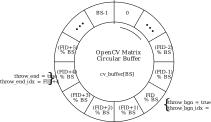
\includegraphics[width=0.9\textwidth]{buffer}
  \caption{OpenCV matrix circular buffer}
  \label{fig:circular_buffer}
\end{figure}

\subsubsection{Image Change Detection}
\label{subsubsec:image_change_detection}
\todo[inline]{Citations, vspace before listings}

% The implementation of the difference computation and the average among all the pixels is described here
% Diff and Mean are done for every frame except the first one (FID = 0)
% Comparison done after the threshold averaging (see chapter threshold)

This section describes the implementation of the image change detection.
The difference computation and the averaging among all the pixels is done for every frame except the first one ($\texttt{FID} \geq 1$).
The threshold comparison and the throw detection is done for every frame after the threshold has been determined (see section \ref{subsubsec:threshold}).

% --------------------------------
\paragraph{Difference Computation}
The absolute difference pixel matrix $D$ can be calculated using equation \ref{eq:abs_diff}.
The implementation uses the OpenCV function \texttt{cv::absdiff} to calculate the per-element absolute difference between the two pixel matrices and saves it into \texttt{cv\_abs}, as shown in appendix \ref{app:throw_detection} on line \ref{lst:ln:abs_diff}.
% https://docs.opencv.org/4.1.1/d2/de8/group__core__array.html#ga6fef31bc8c4071cbc114a758a2b79c14

\begin{equation}
  D = |I_\text{FID} - I_\text{FID-1}| \quad\quad \text{with} \quad\quad \text{FID} \geq 1
  \label{eq:abs_diff}
\end{equation}

\begin{tabular}{rl}
  $D =$ & absolute difference pixel matrix \\
  $I =$ & image pixel matrix \\
\end{tabular}

% --------------------------------------
\paragraph{Average among all the pixels}
The mean absolute difference $\overline{\text{MD}}$ can be calculated using equation \ref{eq:mean_diff}.
The implementation uses the OpenCV function \texttt{cv::sum} to return the sum of array elements for each channel independently, as shown in appendix \ref{app:throw_detection} on line \ref{lst:ln:mean_diff}.
Since the Baumer \texttt{BayerRG8} pixel format consists of only one channel, the zeroth element is used.
% https://docs.opencv.org/4.1.1/d2/de8/group__core__array.html#ga716e10a2dd9e228e4d3c95818f106722

\begin{equation}
  \overline{\text{MD}} = \frac{1}{w\cdot h} \cdot \sum\limits_{i=1}^h \sum\limits_{j=1}^w D_{i,j}
  \label{eq:mean_diff}
\end{equation}

\begin{tabular}{rl}
  $\text{MD} =$ & mean absolute difference \\
  $D =$ & absolute difference pixel matrix \\
  $w =$ & width of the image in px \\
  $h =$ & height of the image in px \\
\end{tabular}

% --------------------------------------------------
\paragraph{Threshold Comparison and Throw Detection}
Listing \ref{lst:throw_detection} shows the implementaion of the threshold comparison and the throw detection.
Due to the specific implementation, it is possible to detect a single frame change.
This means that the image changes between two consecutive frames and then stays the way it is (e.g. sudden change of the ambient light).
Such a glitch is not a valid throw and shall therefore be ignored (see line \ref{lst:ln:glitch_removal}).
Figure \ref{subfig:algorithm_example_1} shows that a valid throw of an object would create at least two changes between individual frames.
The first one by entering and the second one by leaving the frame.
\vspace{5pt}
\begin{lstlisting}[style=C++, caption={Throw detection and glitch removal}, label=lst:throw_detection]
  if (mean_diff >= threshold) {
      if (!throw_bgn) {
        throw_bgn_idx = frame_id;
        throw_bgn = true;
      }
  } else {
    if (throw_bgn) {
      throw_end_idx = frame_id;

      // Remove glitches (single frame changes)
      if ((throw_end_idx - throw_bgn_idx) == 1) {(*\label{lst:ln:glitch_removal}*)
        throw_bgn = false;
      } else {
        throw_end = true;
      }
    }
  }
\end{lstlisting}

As long as no throw is detected, the current Baumer \texttt{Buffer} object is released after each processed frame (see listing \ref{lst:buffer_release}).
Whenever a glitch is removed, the size of the Baumer image buffer (\texttt{BS}) is reduced by one.
This is due to the fact that no reference to past \texttt{Buffer} objects is kept.
Such a reference is necessary to release the respective buffer entry.
It would be easy to solve this by keeping track of at least one past \texttt{Buffer} object.
However, this is not necessary, provided that the buffer size is large enough.
\vspace{5pt}
% BUG: Should not be released directly but with a delay of one!
\begin{lstlisting}[style=C++, caption={Release of the filled Baumer \texttt{Buffer} object}, label=lst:buffer_release]
  if (!throw_bgn) {
    pBufferFilled->QueueBuffer();
  }
\end{lstlisting}





% The implementation of the difference computation and the average among all the pixels is shown in listing \ref{lst:diff_computation_average}.

% \begin{lstlisting}[style=C++, caption={Difference computation and average among all the pixels}, label=lst:diff_computation_average]
%   cv::absdiff(cv_buffer[frame_id % buff_size], cv_buffer[(frame_id - 1) % buff_size], cv_abs);(*\label{lst:ln:abs_diff}*)
%   mean_diff = cv::sum(cv_abs)[0] / (width * height);(*\label{lst:ln:mean_diff}*)
% \end{lstlisting}

\subsubsection{Threshold Value Determination}
\label{subsubsec:threshold}
% \todo[inline]{Citations, Cut in y-axis (not to scale)!}

% how is the Threshold Value Determination done:
% average difference to obtain threshold (with pictures)
    % => 50 Hz flicker reduction

\begin{figure}[H]
  \centering
  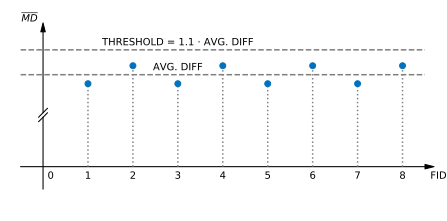
\includegraphics[width=0.75\textwidth]{threshold}
  \caption{Derivation of the threshold value from eigth averaged differences} % 
  \label{fig:threshold}
\end{figure}

\subsubsection{Saving Images}
\label{subsubsec:saving_images}
% \todo[inline]{Citations, Why PNG and not BMP or JPG?}

Resulting in the file names `\texttt{$\{0..(N-1)\}$.png}' (with $N$ beeing the amount of valid frames).

\begin{lstlisting}[style=C++]
  for (int i = throw_bgn_idx; i < (throw_end_idx - 1); ++i) {
    cv::cvtColor(cv_buffer[i % buff_size], cv_transformed, cv::COLOR_BayerBG2BGR);
    cv::imwrite(output_path + std::to_string(i - throw_bgn_idx) + ".png", cv_transformed);
  }
\end{lstlisting}


\subsection{Database}
\label{subsec:database}

All images contain their respective labels in the file name.
This is useful for manually going through them, but not optimal for a program.
The program would have to crawl the directory containing the images and parse the file names.
This requires file system related operations, which are usually very slow.
The solution is to use a database that is designed to read and write such data.
For this reason, a MySQL database is used to store the labels, file names and other metadata.
Table \ref{tab:tab_frames_structure} lists all columns of the database table \texttt{aionfpga.frames}.

\begin{table}[hb]
  \caption{Structure of the database table \texttt{aionfpga.frames}}
  \label{tab:tab_frames_structure}
  \centering
  \begin{tabular}{llll}
    \toprule
    \textbf{Column} & \textbf{Type} & \textbf{Length} & \textbf{Description} \\
    \midrule
    id & \texttt{INT} &  & Sequence number (unique identifier) \\
    timestamp & \texttt{INT} &  & The Unix timestamp at the time of the throw \\
    throwid & \texttt{INT} &  & Throw sequence number \\
    frameid & \texttt{INT} &  & Frame sequence number within a throw \\
    frame & \texttt{VARCHAR} & 255 & The file name of the frame \\
    object & \texttt{VARCHAR} & 255 & The name of the object in the frame (label) \\
    framegood & \texttt{INT} &  & \texttt{0}: frame unusable | \texttt{1}: frame usable \\
    partial & \texttt{INT} &  & \texttt{0}: object fully visible | \texttt{1}: object partially visible \\
    \bottomrule
  \end{tabular}
\end{table}

\clearpage
\subsection{Python Scripts}
\label{subsec:python_scripts}

% creation of the data acquisition and alteration (daa) module with settings and definitions (functions)
% short summary of the function of each python script

This sections lists the various Python scripts and describes their functionality.
Furthermore, it describes the created \textit{Data Acquisition and Alteration} (DAA) Python module.

Collecting and working with a large dataset is not trivial.
% It requires a lot of repetitive taskt, such as moving the files around and chaning the file names.
It requires a lot of repetitive taskt, such as moving files around and chaning file names.
This is very error-prone when performed manually.
To minimize errors, the Python scripts listed in table \ref{tab:python_scripts} werde used.
\\

\paragraph{DAA Python Module}
The different Python scripts require a lot of similar functionality (e.g. database connectivity, printing to the console and handling user input).
For this reason the DAA Python module --- containing settings and definitions (functions) --- was created.
% It contains setting and definitions (functions).
% The usage of classes would not have proven useful
The use of classes did not prove to be beneficial.
Virtually all methods would have to be declared as static methods and therefore regular functions were used.
% Therefore, regular functions were used.

\begin{table}[hb]
  \caption{Description of the various Python scripts}
  \label{tab:python_scripts}
  \centering
  \begin{tabular}{lp{9cm}}
    \toprule
    \textbf{File Name} & \textbf{Description} \\
    \midrule
    \texttt{aionfpga\_daa.py} & This Python script is used to collect the dataset. It runs the \texttt{camera-interface} binary and provides the ability to directly label the frames after each throw. \\
    \midrule
    \texttt{aionfpga\_review\_labels.py} & Even when using Python scripts, the labels have to be selected from a list and human errors might occur. This Python script is used to review the label of each throw and change it, if necessary. \\
    \midrule
    \texttt{aionfpga\_partial\_frames.py} & This Python script is used to go over each throw and to assist the labeling of frames where the object is only partially visible. \\
    \midrule
    \texttt{aionfpga\_stats.py} & During data collection and in the end, it is advantageous to keep an eye on the statistics. This is exactly what this Python script does. \\
    \midrule
    \texttt{aionfpga\_db\_backup.py} & This Python script exports all rows of the database table \texttt{aionfpga.frames} and saves them to a \texttt{.csv} file. \\
    \midrule
    \texttt{aionfpga\_fix\_frameid.py} & Due to different ways of listing files between Windows and the \texttt{os} Python module, the frames were labeled in the wrong order. This Python script is used to undo the complicated transformation. \\
    \bottomrule
  \end{tabular}
\end{table}

% This Python script creates a complete backup of the database table \texttt{aionfpga.frames} and saves it as a \texttt{.csv} file.

